\section{Differenzialrechnung I}
\subsection{Durchschnittliche Änderungsrate}
\subsubsection{Einführungsaufgabe}
Eine Rangierlokomotive bewegt sich entlang der Geleise vor- und rückwärts.
\begin{center}
    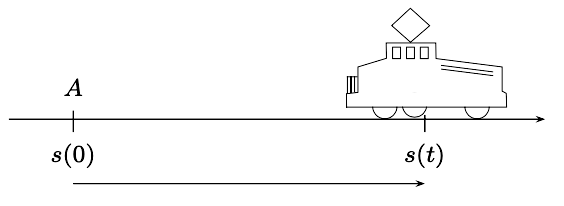
\includegraphics[width=0.25\textwidth]{im/rangierlok.png}

\end{center}

Das folgende „Weg-Zeit-Diagramm“ beschreibt die Bewegung der Lokomotive während 2 Minuten.
Auf der horizontalen Achse ist die Zeit in Sekunden dargestellt. Auf der vertikalen Achse ist der Abstand in Metern von einem Bezugspunkt A auf den Geleisen angegeben. Der Zeitpunkt $t=0$ ist der Moment, in welchem die Lok den Punkt A passiert.
\begin{center}
    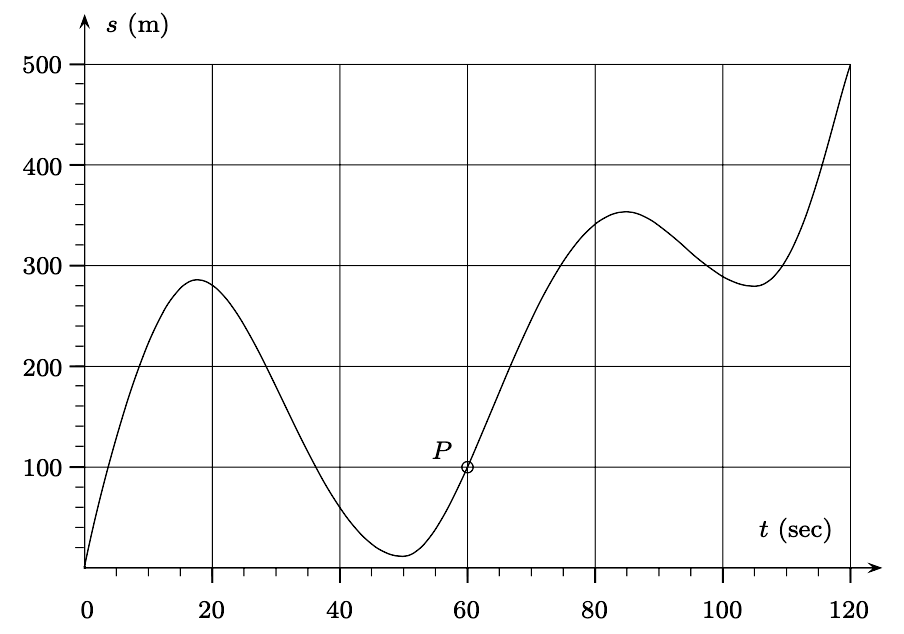
\includegraphics[width=0.6\textwidth]{im/LokWegZeit.png}
\end{center}
\begin{enumerate}
    \item Zu welchen Zeitpunkten befindet sich die Lok 200 Meter vom Punkt A entfernt?
    \item In welchen Zeitintervallen fährt die Lok rückwärts?
    \item Nach 60 Sekunden ist die Lok ungefähr 100m vom Punkt A entfernt. Wie viele Meter ungefähr hat sie \textbf{insgesamt} zurückgelegt?
    \item Berechnen Sie ungefähr die durchschnittliche Geschwindigkeit der Lok während den ersten 10 Sekunden.
    \item Berechnen Sie ungefähr $\frac{s(40)-s(20)}{40-20}$. Was für eine physikalische Bedeutung hat das Resultat und wieso ist es negativ?
    \item Schätzen Sie: Wann fährt die Lok am langsamsten? Wann am schnellsten?
\end{enumerate}
\newpage
\subsubsection{Protokollierung von Bewegungen}
In der Differenzialrechnung geht es darum, dynamische Grössen (wie etwa Position, Geschwindigkeit und Beschleunigung bei bewegten Objekten) rechnerisch zu erfassen und zu analysieren.

Um das Ganze zu vereinfachen, stellen wir uns die bewegten Objekte als Punkte vor. Diese bewegen sich entlang einer Linie. Wir zeichnen meistens eine Gerade, aber die Linie kann auch gekrümmt sein.
\begin{center}
    \begin{tikzpicture}[
        thick,
        every path/.style={line width=1.2pt},
        dot/.style={circle, fill=red, inner sep=0pt, minimum size=6pt},
        arrow/.style={-{Stealth[length=4pt,width=3pt]}, line width=0.8pt}
        ]

        % ── Left figure: straight steep slope ──────────────────────────────────────
        \begin{scope}[shift={(0,0)}]
            % Slope line (angled ~30° from horizontal, going upper-right)
            \draw (-2.2,-1.1) -- (2.2, 1.1);

            % Red dot on the line
            \coordinate (P) at (0, 0.25);
            \node[dot] at (P) {};

            % Two arrows along the slope, pointing away from dot (tangent direction)
            % Direction vector of slope: (2, 1), normalised roughly
            \pgfmathsetmacro{\dx}{0.55}
            \pgfmathsetmacro{\dy}{0.275}
            % arrow to upper-right
            \draw[arrow] (P) -- +(\dx, \dy);
            % arrow to lower-left (reversed)
            \draw[arrow] (P) -- +(-\dx, -\dy);
        \end{scope}

        % ── Right figure: parabola ─────────────────────────────────────────────────
        \begin{scope}[shift={(5.5,0)}]
            % Parabola: y = x^2/2 - 2, drawn from x=-2 to x=2.2
            % Shifted so it looks like the image (opening upward, narrow)
            \draw[samples=100, domain=-1.9:1, smooth]
            plot (\x, {0.7*\x*\x - 1.8});
            \draw[samples=100, domain=1:3, smooth]
            plot (\x, {1.4*\x - 2.5}); % straight line to the right to match the image


            % Point on the right branch, roughly at x=1.5
            \coordinate (Q) at (1.5, 0.1);
            \node[dot] at (Q) {};

            % Tangent direction at x=1.5: slope = 2*0.7*1.5 = 2.1
            % Direction vector (1, 2.1), normalised
            \pgfmathsetmacro{\tx}{0.5}
            \pgfmathsetmacro{\ty}{0.7}
            % single arrow pointing upper-right along tangent
            \draw[arrow] (Q) -- +(\tx, \ty);
            \draw[arrow] (Q) -- +(-\tx, -\ty);
            % small tail (no arrowhead)
            \draw[line width=0.8pt] (Q) -- +(-\tx, -\ty);
        \end{scope}
    \end{tikzpicture}
\end{center}
In beiden Fällen fassen wir die Bewegung als eine eindimensionale auf.

Nun müssen wir die Bewegung unseres Punktes irgendwie protokollieren. Dazu denken wir uns ein Massband entlang der Linie ausgelegt, auf dem wir die Position des Punktes ablesen können. Wir können auch eine Uhr daneben stellen, um die Zeit zu messen.
\begin{center}
    \begin{tikzpicture}[
        thick,
        every path/.style={line width=1.2pt},
        dot/.style={circle, fill=red, inner sep=0pt, minimum size=6pt},
        arrow/.style={-{Stealth[length=4pt,width=3pt]}, line width=0.8pt}
        ]

        \begin{scope}[shift={(0,0)}, rotate=27]
            % Slope line (now drawn horizontally in rotated frame)
            \draw (-2.2, 0) -- (2.2, 0);

            % Red dot on the line
            \coordinate (P) at (-1, 0.5);
            \node[dot] at (P) {};

            % Arrows along line
            \draw[arrow] (P) -- +(0.6, 0);
            \draw[arrow] (P) -- +(-0.6, 0);

            % ── Massband below the line ──
            \def\rulerY{-0.55}      % y-position of ruler top edge
            \def\rulerH{0.22}       % height of ruler box
            \def\rulerL{-1.8}       % left end
            \def\rulerR{1.8}        % right end

            % Ruler box outline
            \draw[line width=0.7pt, fill=white]
            (\rulerL, \rulerY) rectangle (\rulerR, \rulerY-\rulerH);

            % Major ticks every 0.6 units (= 1 unit label), minor every 0.2
            % We go from -1.8 to 1.8 in steps of 0.2
            \foreach \x in {-1.8,-1.6,...,1.8} {
                    \draw[line width=0.5pt]
                    (\x, \rulerY) -- (\x, \rulerY - 0.10);  % minor tick
                }
            % Major ticks every 0.6, with labels  0,1,2,3,4,5,6
            \foreach \i/\lbl in {0/0, 1/1, 2/2, 3/3, 4/4, 5/5, 6/6} {
                    \pgfmathsetmacro{\xpos}{\rulerL + \i*0.6}
                    \draw[line width=0.7pt]
                    (\xpos, \rulerY) -- (\xpos, \rulerY - \rulerH);  % major tick (full height)
                    \node[font=\tiny, anchor=north] at (\xpos, \rulerY-\rulerH) {\lbl};
                }
            \node[font=\small, anchor=north] at (-0.5, -2)
            {$t=1$};
        \end{scope}
        \begin{scope}[shift={(5,0)}, rotate=27]
            % Slope line (now drawn horizontally in rotated frame)
            \draw (-2.2, 0) -- (2.2, 0);

            % Red dot on the line
            \coordinate (P) at (0, 0.5);
            \node[dot] at (P) {};

            % Arrows along line
            \draw[arrow] (P) -- +(0.6, 0);
            \draw[arrow] (P) -- +(-0.6, 0);

            % ── Massband below the line ──
            \def\rulerY{-0.55}      % y-position of ruler top edge
            \def\rulerH{0.22}       % height of ruler box
            \def\rulerL{-1.8}       % left end
            \def\rulerR{1.8}        % right end

            % Ruler box outline
            \draw[line width=0.7pt, fill=white]
            (\rulerL, \rulerY) rectangle (\rulerR, \rulerY-\rulerH);

            % Major ticks every 0.6 units (= 1 unit label), minor every 0.2
            % We go from -1.8 to 1.8 in steps of 0.2
            \foreach \x in {-1.8,-1.6,...,1.8} {
                    \draw[line width=0.5pt]
                    (\x, \rulerY) -- (\x, \rulerY - 0.10);  % minor tick
                }
            % Major ticks every 0.6, with labels  0,1,2,3,4,5,6
            \foreach \i/\lbl in {0/0, 1/1, 2/2, 3/3, 4/4, 5/5, 6/6} {
                    \pgfmathsetmacro{\xpos}{\rulerL + \i*0.6}
                    \draw[line width=0.7pt]
                    (\xpos, \rulerY) -- (\xpos, \rulerY - \rulerH);  % major tick (full height)
                    \node[font=\tiny, anchor=north] at (\xpos, \rulerY-\rulerH) {\lbl};
                }
            \node[font=\small, anchor=north] at (-0.5, -2)
            {$t=2$};
        \end{scope}
        \begin{scope}[shift={(10,0)}, rotate=27]
            % Slope line (now drawn horizontally in rotated frame)
            \draw (-2.2, 0) -- (2.2, 0);

            % Red dot on the line
            \coordinate (P) at (1.5, 0.5);
            \node[dot] at (P) {};

            % Arrows along line
            \draw[arrow] (P) -- +(0.6, 0);
            \draw[arrow] (P) -- +(-0.6, 0);

            % ── Massband below the line ──
            \def\rulerY{-0.55}      % y-position of ruler top edge
            \def\rulerH{0.22}       % height of ruler box
            \def\rulerL{-1.8}       % left end
            \def\rulerR{1.8}        % right end

            % Ruler box outline
            \draw[line width=0.7pt, fill=white]
            (\rulerL, \rulerY) rectangle (\rulerR, \rulerY-\rulerH);

            % Major ticks every 0.6 units (= 1 unit label), minor every 0.2
            % We go from -1.8 to 1.8 in steps of 0.2
            \foreach \x in {-1.8,-1.6,...,1.8} {
                    \draw[line width=0.5pt]
                    (\x, \rulerY) -- (\x, \rulerY - 0.10);  % minor tick
                }
            % Major ticks every 0.6, with labels  0,1,2,3,4,5,6
            \foreach \i/\lbl in {0/0, 1/1, 2/2, 3/3, 4/4, 5/5, 6/6} {
                    \pgfmathsetmacro{\xpos}{\rulerL + \i*0.6}
                    \draw[line width=0.7pt]
                    (\xpos, \rulerY) -- (\xpos, \rulerY - \rulerH);  % major tick (full height)
                    \node[font=\tiny, anchor=north] at (\xpos, \rulerY-\rulerH) {\lbl};
                }
            \node[font=\small, anchor=north] at (-0.5, -2)
            {$t=2.5$};
        \end{scope}
    \end{tikzpicture}
\end{center}
So können wir die Position des Punktes zu verschiedenen Zeitpunkten ablesen und auf folgende Weisen protokollieren:
\begin{itemize}
    \item \textbf{Tabellarisch}: Wir können die Zeitpunkte und die entsprechenden Positionen in einer Tabelle festhalten.
    \item \textbf{Graphisch}: Wir können die Positionen als Punkte in einem Koordinatensystem einzeichnen, wobei die horizontale Achse die Zeit und die vertikale Achse die Position darstellt. So erhalten wir ein „Weg-Zeit-Diagramm“.
    \item \textbf{Algebraisch}: Wir können die Position als Funktion der Zeit angeben, also $s(t)$, wobei $s$ die Position und $t$ die Zeit ist. So erhalten wir eine „Weg-Zeit-Funktion“.
\end{itemize}
\begin{example}
    \begin{minipage}{0.35\textwidth}
        \begin{center}
            \begin{tabular}{c|c|c|c|c|c}
                $t$    & 0 & 1   & 2 & 2.5  & $\dots$ \\
                \hline
                $s(t)$ & 2 & 2.5 & 3 & 3.25 & $\dots$
            \end{tabular}
        \end{center}
    \end{minipage}
    \begin{minipage}
        {0.35\textwidth}
        \begin{center}
            \begin{tikzpicture}[
                scale=0.4,
                axis/.style={-{Stealth[length=6pt,width=4pt]}, line width=1pt},
                grid/.style={line width=0.3pt, color=gray!40},
                thick line/.style={line width=1.5pt},
                ]

                % ── Grid ──────────────────────────────────────────────────────────────────
                \draw[grid] (-5,-1) grid (8,7);

                % ── Axes ──────────────────────────────────────────────────────────────────
                \draw[axis] (-5,0) -- (8.4,0) node[right, font=\tiny\itshape] {$t$};
                \draw[axis] (0,-1) -- (0,7.4) node[above, font=\tiny\itshape] {$s(t)$};

                % ── Tick marks and labels – x axis ────────────────────────────────────────
                \foreach \x in {-5,-4,-3,-2,-1,1,2,3,4,5,6,7,8} {
                        \draw[line width=0.6pt] (\x, 0.07) -- (\x, -0.07);
                        \node[font=\tiny, anchor=north, inner sep=2pt] at (\x, 0) {\x};
                    }

                % ── Tick marks and labels – y axis ────────────────────────────────────────
                \foreach \y in {-1,1,2,3,4,5,6} {
                        \draw[line width=0.6pt] (0.07, \y) -- (-0.07, \y);
                        \node[font=\tiny, anchor=east, inner sep=2pt] at (0, \y) {\y};
                    }

                % ── Origin label ──────────────────────────────────────────────────────────
                \node[font=\tiny, anchor=north east, inner sep=2pt] at (0,0) {0};

                % ── Red line: passes through (0,2) with slope ~0.5, i.e. s(t)=0.5t+2 ──
                % From the image: at t=-5 => ~-0.75, at t=8 => ~6.4
                % Slope ≈ (6.4 - (-0.75))/(8-(-5)) = 7.15/13 ≈ 0.5
                \draw[red, line width=1.0pt] (-5, {0.5*(-5)+2}) -- (8, {0.5*8+2});
            \end{tikzpicture}
        \end{center}
    \end{minipage}
    \begin{minipage}
        {0.25\textwidth}
        \[
            s(t) = 0.5 t + 2
        \]
    \end{minipage}
\end{example}
\begin{example}
    \begin{minipage}{0.35\textwidth}
        \begin{center}
            \begin{tabular}{c|c|c|c|c|c}
                $t$    & 0 & 1 & 2 & 2.5 & $\dots$ \\
                \hline
                $s(t)$ & 3 & 3 & 3 & 3   & $\dots$
            \end{tabular}
        \end{center}
    \end{minipage}
    \begin{minipage}
        {0.35\textwidth}
        \begin{center}
            \begin{tikzpicture}[
                scale=0.4,
                axis/.style={-{Stealth[length=6pt,width=4pt]}, line width=1pt},
                grid/.style={line width=0.3pt, color=gray!40},
                thick line/.style={line width=1.5pt},
                ]

                % ── Grid ──────────────────────────────────────────────────────────────────
                \draw[grid] (-5,-1) grid (8,7);

                % ── Axes ──────────────────────────────────────────────────────────────────
                \draw[axis] (-5,0) -- (8.4,0) node[right, font=\tiny\itshape] {$t$};
                \draw[axis] (0,-1) -- (0,7.4) node[above, font=\tiny\itshape] {$s(t)$};

                % ── Tick marks and labels – x axis ────────────────────────────────────────
                \foreach \x in {-5,-4,-3,-2,-1,1,2,3,4,5,6,7,8} {
                        \draw[line width=0.6pt] (\x, 0.07) -- (\x, -0.07);
                        \node[font=\tiny, anchor=north, inner sep=2pt] at (\x, 0) {\x};
                    }

                % ── Tick marks and labels – y axis ────────────────────────────────────────
                \foreach \y in {-1,1,2,3,4,5,6} {
                        \draw[line width=0.6pt] (0.07, \y) -- (-0.07, \y);
                        \node[font=\tiny, anchor=east, inner sep=2pt] at (0, \y) {\y};
                    }

                % ── Origin label ──────────────────────────────────────────────────────────
                \node[font=\tiny, anchor=north east, inner sep=2pt] at (0,0) {0};

                % ── Red line: passes through (0,2) with slope ~0.5, i.e. s(t)=0.5t+2 ──
                % From the image: at t=-5 => ~-0.75, at t=8 => ~6.4
                % Slope ≈ (6.4 - (-0.75))/(8-(-5)) = 7.15/13 ≈ 0.5
                \draw[red, line width=1.0pt] (-5, 3) -- (8, 3);
            \end{tikzpicture}
        \end{center}
    \end{minipage}
    \begin{minipage}
        {0.25\textwidth}
        \[
            s(t) = 3
        \]
    \end{minipage}
\end{example}
\begin{example}
    \begin{minipage}{0.35\textwidth}
        \begin{center}
            \begin{tabular}{c|c|c|c|c|c}
                $t$    & 0 & 1    & 2 & 3    & $\dots$ \\
                \hline
                $s(t)$ & 2 & 2.25 & 3 & 4.25 & $\dots$
            \end{tabular}
        \end{center}
    \end{minipage}
    \begin{minipage}
        {0.35\textwidth}
        \begin{center}
            \begin{tikzpicture}[
                scale=0.4,
                axis/.style={-{Stealth[length=6pt,width=4pt]}, line width=1pt},
                grid/.style={line width=0.3pt, color=gray!40},
                thick line/.style={line width=1.5pt},
                ]

                % ── Grid ──────────────────────────────────────────────────────────────────
                \draw[grid] (0,0) grid (8,7);

                % ── Axes ──────────────────────────────────────────────────────────────────
                \draw[axis] (0,0) -- (8.4,0) node[right, font=\tiny\itshape] {$t$};
                \draw[axis] (0,0) -- (0,7.4) node[above, font=\tiny\itshape] {$s(t)$};

                % ── Tick marks and labels – x axis ────────────────────────────────────────
                \foreach \x in {1,2,3,4,5,6,7,8} {
                        \draw[line width=0.6pt] (\x, 0.07) -- (\x, -0.07);
                        \node[font=\tiny, anchor=north, inner sep=2pt] at (\x, 0) {\x};
                    }

                % ── Tick marks and labels – y axis ────────────────────────────────────────
                \foreach \y in {1,2,3,4,5,6} {
                        \draw[line width=0.6pt] (0.07, \y) -- (-0.07, \y);
                        \node[font=\tiny, anchor=east, inner sep=2pt] at (0, \y) {\y};
                    }

                % ── Origin label ──────────────────────────────────────────────────────────
                \node[font=\tiny, anchor=north east, inner sep=2pt] at (0,0) {0};

                % ── Red parabola: s(t) = 1/2 * 7 * t^2 + 3 = 3.5t^2 + 3 ─────────────────
                % Clipped to visible window
                \clip (0,0) rectangle (8,7);
                \draw[red, line width=1.8pt, samples=200, domain=0:8, smooth]
                plot (\x, {0.25*\x*\x + 2});
            \end{tikzpicture}
        \end{center}
    \end{minipage}
    \begin{minipage}
        {0.25\textwidth}
        \[
            s(t) = \dfrac{1}{4}\cdot t^2 + 2
        \]
    \end{minipage}
\end{example}
Solange sich das Objekt immer vorwärts bewegt (d.h. in positiver Richtung des Massbandes), können wir den vom Zeitpunkt $t_1$ bis $t_2$ zurückgelegten Weg einfach als die Differenz der Positionen zu zwei Zeitpunkten berechnen:
\[
    \text{Positionsänderung} = s(t_2) - s(t_1)
\]
\begin{example}
    Vorsicht, die Positionsänderung ist nicht immer gleichbedeutend mit der zurückgelegten Strecke. Gegenbeispiel: $s(t)=\sin(t)$

    \begin{minipage}{0.3\textwidth}
        \begin{center}
            \begin{tikzpicture}[
                scale=0.4,
                axis/.style={-{Stealth[length=6pt,width=4pt]}, line width=1pt},
                grid/.style={line width=0.3pt, color=gray!40},
                thick line/.style={line width=1.5pt},
                ]

                % ── Grid ──────────────────────────────────────────────────────────────────
                \draw[grid] (-1,-1) grid (8,3);

                % ── Axes ──────────────────────────────────────────────────────────────────
                \draw[axis] (-1,0) -- (8.4,0) node[right, font=\tiny\itshape] {$t$};
                \draw[axis] (0,-1) -- (0,2.8) node[above, font=\tiny\itshape] {$s(t)$};

                % ── Tick marks and labels – x axis ────────────────────────────────────────
                \foreach \x in {1,2,3,4,5,6,7,8} {
                        \draw[line width=0.6pt] (\x, 0.07) -- (\x, -0.07);
                        \node[font=\tiny, anchor=north, inner sep=2pt] at (\x, 0) {\x};
                    }

                % ── Tick marks and labels – y axis ────────────────────────────────────────
                \foreach \y in {-1,1,2,3} {
                        \draw[line width=0.6pt] (0.07, \y) -- (-0.07, \y);
                        \node[font=\tiny, anchor=east, inner sep=2pt] at (0, \y) {\y};
                    }

                % ── Origin label ──────────────────────────────────────────────────────────
                \node[font=\tiny, anchor=north east, inner sep=2pt] at (0,0) {0};

                % ── Red parabola: s(t) = 1/2 * 7 * t^2 + 3 = 3.5t^2 + 3 ─────────────────
                % Clipped to visible window
                \clip (0,-1.5) rectangle (8,3);
                \draw[red, line width=1.8pt, samples=200, domain=0:8, smooth]
                plot (\x, {sin(\x r)});
            \end{tikzpicture}
        \end{center}
    \end{minipage}
    \begin{minipage}{0.7\textwidth}
        und die Zeitpunkte $t_1=0$ und $t_2=2\pi$.

        $s(t_2)-s(t_1)=\sin(2\pi)-\sin(0)=0-0=0$, obwohl die zurückgelegte Strecke offensichtlich nicht 0 ist.
    \end{minipage}
    \label{ex:avgspeedzero}
\end{example}
\subsubsection{Von der Durchschnittsgeschwindigkeit zur durchschnittlichen Änderungsrate}
$\dfrac{s(t_2)-s(t_1)}{t_2-t_1}$ sagt uns, um wie viel sich die Position im Zeitintervall $[t_1,t_2]$ durchschnittlich ändert. Wir nennen dies auch die \textbf{Durchschnittsgeschwindigkeit} im Zeitintervall $[t_1,t_2]$. Diese kann $0$ sein, auch wenn die zurückgelegte Strecke nicht $0$ ist (siehe Beispiel \ref{ex:avgspeedzero}).

Etwas allgemeiner spricht man von der \textbf{durchschnittlichen Änderungsrate} der Position im Zeitintervall $[t_1,t_2]$. Denn sie gibt an, um wie viel sich die Position durchschnittlich ändert, wenn sich die Zeit um eine Einheit ändert. Dies lässt sich auf allgemeine Funktionen übertragen:

\begin{deff}[Durchschnittliche Änderungsrate]{}
    Die \textbf{durchschnittliche Änderungsrate} einer Funktion $f$ im Intervall $[a,b]$ ist gegeben durch:
    \[
        \frac{f(b)-f(a)}{b-a}
    \]
    Sie gibt an, um wie viel sich die Funktion $f$ im Intervall $[a,b]$ pro Einheit durchschnittlich ändert.
\end{deff}
\begin{example}
    Diesmal gibt die Funktion $v(t)=2t$ die Geschwindigkeit eines Objektes zum Zeitpunkt $t$ an.
    \begin{itemize}
        \item $v(t_2)-v(t_1)$ gibt an, um wie viel sich die Geschwindigkeit im Zeitintervall $[t_1,t_2]$ ändert.

        \item $\dfrac{v(t_2)-v(t_1)}{t_2-t_1}$ gibt an, um wie viel sich die Geschwindigkeit im Zeitintervall $[t_1,t_2]$ pro Zeiteinheit durchschnittlich ändert. Das ist die durchschnittliche Änderungsrate der Geschwindigkeit, also die durchschnittliche Beschleunigung im Intervall $[t_1,t_2]$.
    \end{itemize}
\end{example}
\begin{example}
    Während den zehn Minuten, in denen ein Ofen auf $200^\circ C$ erhitzt wird, verläuft die Temperatur nach der Gleichung:
    \[
        T(t) = -\frac{9}{5} (t-10)^2 + 200
    \]
    wobei $t$ die Zeit in Minuten und $T$ die Temperatur in $^\circ C$ angibt.

    \begin{center}
        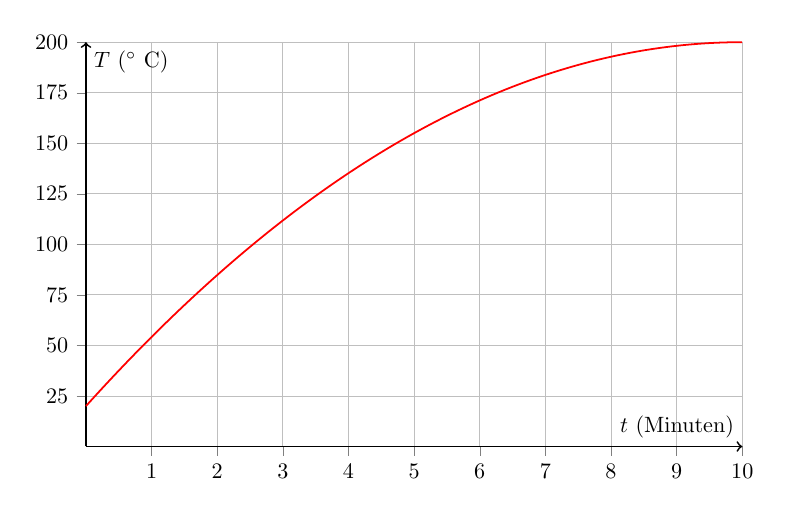
\begin{tikzpicture}[scale=0.8]
            \begin{axis}[
                    width=12cm, height=8cm,
                    grid=major,
                    xlabel={$t$ (Minuten)},
                    ylabel={$T$ ($^\circ$ C)},
                    xmin=0, xmax=10,
                    ymin=0, ymax=200,
                    xtick={0,1,2,3,4,5,6,7,8,9,10},
                    ytick={0,25,50,75,100,125,150,175,200},
                    domain=0:10,
                    samples=100,
                    thick,
                    smooth,
                    axis lines=middle,
                    axis line style={->},
                    enlargelimits=false,
                    clip=false,
                    tick align=outside
                ]
                \addplot[red, thick] {-9/5*(x-10)^2 + 200};
            \end{axis}
        \end{tikzpicture}
    \end{center}
    \begin{itemize}
        \item $T(t_2)-T(t_1)$ gibt an, um wie viel sich die Temperatur im Zeitintervall $[t_1,t_2]$ ändert.

              $T(10)-T(1)=200 - 54.2 = 145.8$
        \item $\dfrac{T(t_2)-T(t_1)}{t_2-t_1}$ gibt an, um wie viel sich die Temperatur im Zeitintervall $[t_1,t_2]$ pro Zeiteinheit durchschnittlich ändert. Das ist die durchschnittliche Änderungsrate der Temperatur im Intervall $[t_1,t_2]$.

              $\dfrac{T(10)-T(1)}{10-1}=\dfrac{145.8}{9}=16.2$
    \end{itemize}
\end{example}
\clearpage
\subsubsection{Übungen}
\begin{enumerate}
    \item Ordnen Sie den s-t-Graphen die passendsten sprachlichen Beschreibungen zu.
          % helper style
          \tikzset{
          ax/.style={-{Stealth[length=4pt,width=3pt]}, line width=0.7pt},
          gr/.style={line width=0.25pt, color=gray!40, dashed},
          cu/.style={red!75, line width=1.4pt},
          }

          % ── macro: draw axes + grid, no foreach in newcommand ──────────────────────
          % We inline each graph fully to avoid expansion issues.

          \begin{tikzpicture}[scale=0.58]

              % ─────────────────────────────────────────────────────────────────
              % COLUMN offsets: left=0, right=7.5
              % ROW offsets:   r1=0, r2=-7.5, r3=-15, r4=-22
              % ─────────────────────────────────────────────────────────────────

              %% ══ a) linear s=0.5t ════════════════════════════════════════════
              \begin{scope}[xshift=0cm, yshift=0cm]
                  \draw[gr] (0,-1) grid (7,5);
                  \draw[ax] (-0.2,0)--(7.5,0) node[right,font=\small\it]{$t$};
                  \draw[ax] (0,-1.2)--(0,5.5) node[above,font=\small\it]{$s(t)$};
                  \foreach \x in {1,...,7}{\draw(\x,.05)--(\x,-.05);\node[font=\tiny,below=1pt]at(\x,0){\x};}
                  \foreach \y in {-1,1,2,3,4,5}{\draw(.05,\y)--(-.05,\y);\node[font=\tiny,left=1pt]at(0,\y){\y};}
                  \node[font=\tiny,below left=1pt]at(0,0){0};
                  \node[font=\normalsize,above left=2pt]at(-1,5){a)};
                  \clip(0,-1)rectangle(7,5);
                  \draw[cu](0,0)--(7,3.5);
              \end{scope}

              %% ══ b) decay e^{-0.6t} ═════════════════════════════════════════
              \begin{scope}[xshift=12cm, yshift=0cm]
                  \draw[gr] (0,-1) grid (7,5);
                  \draw[ax] (-0.2,0)--(7.5,0) node[right,font=\small\it]{$t$};
                  \draw[ax] (0,-1.2)--(0,5.5) node[above,font=\small\it]{$s(t)$};
                  \foreach \x in {1,...,7}{\draw(\x,.05)--(\x,-.05);\node[font=\tiny,below=1pt]at(\x,0){\x};}
                  \foreach \y in {-1,1,2,3,4,5}{\draw(.05,\y)--(-.05,\y);\node[font=\tiny,left=1pt]at(0,\y){\y};}
                  \node[font=\tiny,below left=1pt]at(0,0){0};
                  \node[font=\normalsize,above left=2pt]at(-1,5){b)};
                  \clip(0,-1)rectangle(7,5);
                  \draw[cu,samples=120,domain=0.2:7,smooth] plot(\x,{1/(\x)});
              \end{scope}

              %% ══ c) tent: (0,0)->(3,6)->(6,0) ══════════════════════════════
              \begin{scope}[xshift=0cm, yshift=-10cm]
                  \draw[gr] (0,-1) grid (7,6);
                  \draw[ax] (-0.2,0)--(7.5,0) node[right,font=\small\it]{$t$};
                  \draw[ax] (0,-1.2)--(0,6.8) node[above,font=\small\it]{$s(t)$};
                  \foreach \x in {1,...,7}{\draw(\x,.05)--(\x,-.05);\node[font=\tiny,below=1pt]at(\x,0){\x};}
                  \foreach \y in {-1,1,2,3,4,5,6}{\draw(.05,\y)--(-.05,\y);\node[font=\tiny,left=1pt]at(0,\y){\y};}
                  \node[font=\tiny,below left=1pt]at(0,0){0};
                  \node[font=\normalsize,above left=2pt]at(-1,5){c)};
                  \clip(0,-1)rectangle(7,6);
                  \draw[cu](0,0)--(3,6)--(6,0);
              \end{scope}

              %% ══ d) constant s=3 ════════════════════════════════════════════
              \begin{scope}[xshift=12cm, yshift=-10cm]
                  \draw[gr] (0,-1) grid (7,5);
                  \draw[ax] (-0.2,0)--(7.5,0) node[right,font=\small\it]{$t$};
                  \draw[ax] (0,-1.2)--(0,5.5) node[above,font=\small\it]{$s(t)$};
                  \foreach \x in {1,...,7}{\draw(\x,.05)--(\x,-.05);\node[font=\tiny,below=1pt]at(\x,0){\x};}
                  \foreach \y in {-1,1,2,3,4,5}{\draw(.05,\y)--(-.05,\y);\node[font=\tiny,left=1pt]at(0,\y){\y};}
                  \node[font=\tiny,below left=1pt]at(0,0){0};
                  \node[font=\normalsize,above left=2pt]at(-1,5){d)};
                  \clip(0,-1)rectangle(7,5);
                  \draw[cu](0,3)--(7,3);
              \end{scope}

              %% ══ e) quadratic s=0.3t^2 ══════════════════════════════════════
              \begin{scope}[xshift=0cm, yshift=-19cm]
                  \draw[gr] (-1,-1) grid (5,5);
                  \draw[ax] (-1.2,0)--(5.5,0) node[right,font=\small\it]{$t$};
                  \draw[ax] (0,-1.2)--(0,5.5) node[above,font=\small\it]{$s(t)$};
                  \foreach \x in {-1,1,...,5}{\draw(\x,.05)--(\x,-.05);\node[font=\tiny,below=1pt]at(\x,0){\x};}
                  \foreach \y in {-1,1,2,3,4,5}{\draw(.05,\y)--(-.05,\y);\node[font=\tiny,left=1pt]at(0,\y){\y};}
                  \node[font=\tiny,below left=1pt]at(0,0){0};
                  \node[font=\normalsize,above left=2pt]at(-1,5){e)};
                  \clip(-1.2,-1)rectangle(5,5);
                  \draw[cu,samples=100,domain=-1.2:4.08,smooth] plot(\x,{2^(\x-1)});
              \end{scope}

              %% ══ f) sqrt s=2*sqrt(t) ════════════════════════════════════════
              \begin{scope}[xshift=12cm, yshift=-19cm]
                  \draw[gr] (0,-1) grid (7,5);
                  \draw[ax] (-0.2,0)--(7.5,0) node[right,font=\small\it]{$t$};
                  \draw[ax] (0,-1.2)--(0,5.5) node[above,font=\small\it]{$s(t)$};
                  \foreach \x in {1,...,7}{\draw(\x,.05)--(\x,-.05);\node[font=\tiny,below=1pt]at(\x,0){\x};}
                  \foreach \y in {-1,1,2,3,4,5}{\draw(.05,\y)--(-.05,\y);\node[font=\tiny,left=1pt]at(0,\y){\y};}
                  \node[font=\tiny,below left=1pt]at(0,0){0};
                  \node[font=\normalsize,above left=2pt]at(-1,5){f)};
                  \clip(0,-1)rectangle(7,5);
                  \draw[cu,samples=100,domain=0:7,smooth] plot(\x,{2*sqrt(\x)});
              \end{scope}

              %% ══ g) s=t-1, starts at (0,-1), crosses x at t=1 ══════════════
              \begin{scope}[xshift=0cm, yshift=-28cm]
                  \draw[gr] (-0.5,-1.5) grid (4.5,4);
                  \draw[ax] (-0.7,0)--(4.8,0) node[right,font=\small\it]{$t$};
                  \draw[ax] (0,-1.7)--(0,4.5) node[above,font=\small\it]{$s(t)$};
                  \foreach \x in {1,...,4}{\draw(\x,.05)--(\x,-.05);\node[font=\tiny,below=1pt]at(\x,0){\x};}
                  \foreach \y in {-1,1,2,3,4}{\draw(.05,\y)--(-.05,\y);\node[font=\tiny,left=1pt]at(0,\y){\y};}
                  \node[font=\tiny,below left=1pt]at(0,0){0};
                  \node[font=\normalsize,above left=2pt]at(-1,5){g)};
                  \clip(-0.5,-1.5)rectangle(4.5,4);
                  \draw[cu](-1,-3)--(2,6);
              \end{scope}

              %% ══ h) linear decrease s=5-0.5t ════════════════════════════════
              \begin{scope}[xshift=12cm, yshift=-28cm]
                  \draw[gr] (0,0) grid (9,5);
                  \draw[ax] (-0.2,0)--(9.5,0) node[right,font=\small\it]{$t$};
                  \draw[ax] (0,-0.3)--(0,5.5) node[above,font=\small\it]{$s(t)$};
                  \foreach \x in {1,...,9}{\draw(\x,.05)--(\x,-.05);\node[font=\tiny,below=1pt]at(\x,0){\x};}
                  \foreach \y in {1,2,3,4,5}{\draw(.05,\y)--(-.05,\y);\node[font=\tiny,left=1pt]at(0,\y){\y};}
                  \node[font=\tiny,below left=1pt]at(0,0){0};
                  \node[font=\normalsize,above left=2pt]at(-1,5){h)};
                  \clip(0,0)rectangle(9,5);
                  \draw[cu](0,5)--(8,1);
              \end{scope}

          \end{tikzpicture}
          \begin{enumerate}[label=(\roman*)]
              \item bewegt sich nicht
              \item bewegt sich schnell und mit konstanter Geschwindigkeit vorwärts. \item bewegt sich beschleunigt vorwärts.
              \item bewegt sich mit konstanter Geschwindigkeit rückwärts.
              \item bewegt sich langsam und mit konstanter Geschwindigkeit vorwärts. \item fährt gleichförmig vorwärts, kehrt um und fährt dann gleichförmig rückwärts.
              \item bewegt sich langsamer werdend vorwärts.
              \item nähert sich rückwärtsfahrend sehr schnell dem Ort 0 und bremst dann stark ab.
          \end{enumerate}
    \item Begründen Sie, weshalb folgende Behauptung falsch ist: \glqq $s(t)$ gibt immer die Länge der Wegstrecke an, die nach $t$ Zeiteinheiten zurückgelegt wurde.\grqq
    \item Wenn man einen s-t-Graphen vor sich hat, woran erkennt man auf einen Blick, ob es sich um eine gleichförmige Bewegung (mit konstanter Geschwindigkeit) handelt oder nicht?
    \item Stellen Sie die folgenden Bewegungen je durch eine Bewegungsgleichung dar:
          \begin{enumerate}
              \item Das Objekt bewegt sich gleichförmig 3 Einheiten pro Zeiteinheit vorwärts und passiert zum Zeitpunkt $0$ die Position $0$.
              \item Das Objekt bewegt sich gleichförmig 5 Einheiten pro Zeiteinheit rückwärts und passiert zum Zeitpunkt $0$ die Position $3$.
              \item Das Objekt bewegt sich gleichförmig 1 Einheit pro Zeiteinheit vorwärts und passiert zum Zeitpunkt $5$ die Position $2$.
          \end{enumerate}
    \item Richtig oder falsch? Begründen Sie oder geben Sie ein Gegenbeispiel an: \glqq Wenn die durchschnittliche Änderungsrate einer Funktion $f$ im Intervall $[a,b]$ gleich $2$ ist, dann nimmt $f$ im Intervall $[a,b]$ pro Einheit um 2 zu.\grqq
    \item Geben Sie für die folgenden Grössen und deren abhängige Variable die Interpretation der durchschnittlichen Änderungsrate an. Beispiel: $T(t)$ Temperatur des Ofens zum Zeitpunkt $t$ in Minuten. Interpretation: Die durchschnittliche Temperaturänderung pro Minute.
          \begin{enumerate}
              \item $K(t)$ Kontostand zum Zeitpunkt $t$ in Tagen.
              \item Höhe $h(t)$ eines Ballons in Metern abhängig von der Zeit t in s.
              \item $P(t)$ Preis eines Produkts zum Zeitpunkt $t$ in Tagen. Interpretation: Die durchschnittliche Preisänderung pro Tag.
              \item Verbrauchte Liter Benzin $V(s)$ eines Autos nach $s$ zurückgelegten Kilometern.
          \end{enumerate}
\end{enumerate}
\newpage
\subsubsection*{Lösungen}
\begin{enumerate}
    \item (a) (v), (b) (viii), (c) (vi), (d) (i), (e) (iii), (f) (vii), (g) (ii), (h) (iv)
    \item Falsch, siehe Beispiel \ref{ex:avgspeedzero}. $s(t)$ gibt die Position an, nicht die zurückgelegte Strecke. Wenn sich das Objekt vorwärts und rückwärts bewegt, kann die Position gleich bleiben, obwohl eine Strecke zurückgelegt wurde.
    \item An der Form des Graphen: Ein s-t-Graph einer gleichförmigen Bewegung ist eine Gerade, da die Position sich mit konstanter Geschwindigkeit ändert. Wenn der Graph eine Kurve ist, handelt es sich nicht um eine gleichförmige Bewegung.
    \item \begin{enumerate}
              \item $s(t) = 3t$
              \item $s(t) = 3 - 5t$
              \item $s(t) = 2 + (t-5) = t - 3$
          \end{enumerate}
    \item Falsch. Die durchschnittliche Änderungsrate gibt an, um wie viel sich die Funktion \textbf{im Durchschnitt} pro Einheit ändert, aber das bedeutet nicht, dass die Funktion tatsächlich pro Einheit um genau diesen Betrag zunimmt. Es könnte zum Beispiel sein, dass die Funktion in der ersten Hälfte des Intervalls stark zunimmt und in der zweiten Hälfte stark abnimmt, sodass die durchschnittliche Änderungsrate 2 ist, obwohl die Funktion nicht konstant um 2 pro Einheit zunimmt.
    \item
          \begin{enumerate}
              \item durchschnittliche Änderungsrate: durchschnittliche Zu- oder Abnahme des Guthabens pro Monat, sprich durchschnittliche Einnahmen oder Ausgaben pro Monat.
              \item durchschnittliche Änderungsrate: durchschnittliche Steig- oder Sinkgeschwindigkeit in m/s
              \item durchschnittliche Änderungsrate: durchschnittliche Preisänderung pro Tag.
              \item durchschnittliche Änderungsrate: durchschnittlicher Verbrauch pro Kilometer in Litern pro Kilometer.
          \end{enumerate}
\end{enumerate}
\newpage
\subsection{Differenzenquotient und Differenzialquotient}
\subsubsection{Einführungsaufgabe}
Auf der 100-Meter-Bahn der KS Im Lee wird ein Roboter getestet. Er wird auf die Startlinie gesetzt und beschleunigt schnell in Richtung Ziellinie. Der Roboter wird so programmiert, dass er sich gemäss der folgenden Bewegungsgleichung bewegt:
\[
    s(t) = \frac{1}{4} t^2
\]
Das bedeutet, dass der Roboter nach $t$ Sekunden die Strecke $s(t) = \frac{1}{4} t^2$ in Metern zurückgelegt hat. Wir denken uns entlang der Bahn ein Messband ausgelegt, sodass wir immer die Position des Roboters in Metern nach dem Startpunkt ablesen können.
\begin{enumerate}
    \item Skizziere den Graphen der Funktion $s(t)$ im Bereich $0 \leq t \leq 8$.
          \begin{center}
              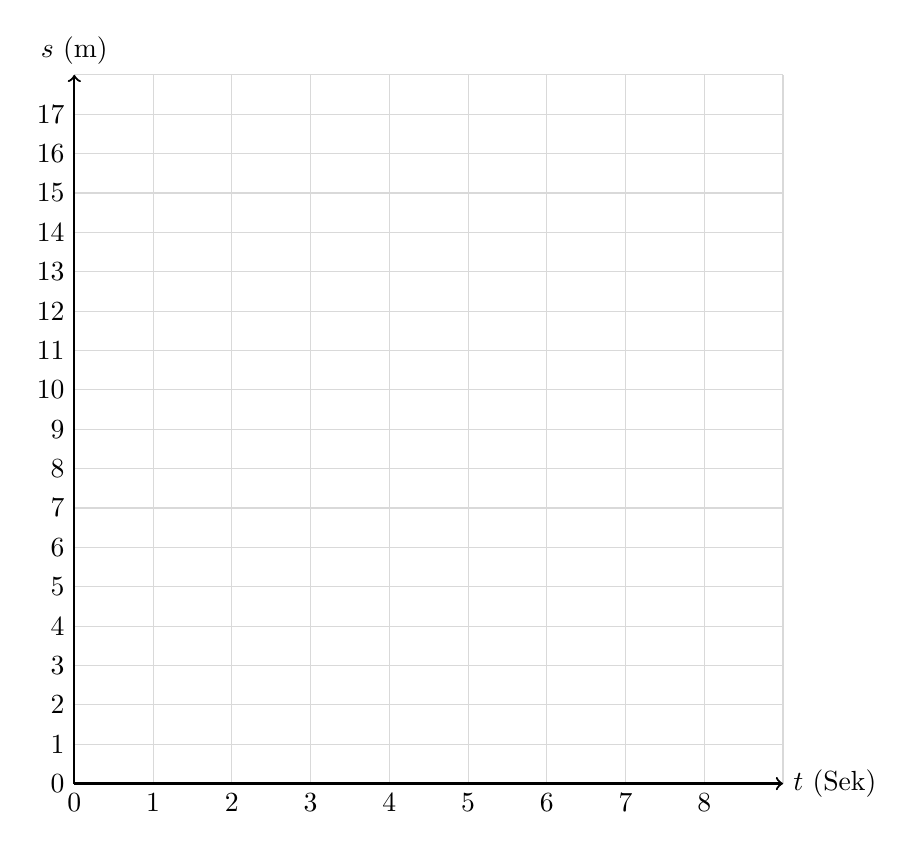
\begin{tikzpicture}


                  % Rasterlinien
                  % \draw[gray!30, step=1] (0,0) grid (8,9);
                  \draw[gray!30,xstep=1, ystep=0.5] (0,0) grid (9,9);  % X-Richtung (Schrittweite 1)
                  %\draw[gray!30,step=0.5,ystep=0.5] (0,0) grid (9,9);  % Y-Richtung (Schrittweite 0.5)
                  % Achsen
                  \draw[->, thick] (0,0) -- (9,0) node[right] {$t$ (Sek)};
                  \draw[->, thick] (0,0) -- (0,9) node[above] {$s$ (m)};

                  % Beschriftungen der Achsen
                  \foreach \x in {0,1,2,3,4,5,6,7,8} {
                          \node[below] at (\x,0) {\x };
                      }
                  \foreach \y in {0,1,2,3,4,5,6,7,8,9,10,11,12,13,14,15,16,17} {
                          \node[left] at (0,\y/2) {\y };
                      }
              \end{tikzpicture}
          \end{center}


    \item Welche Position lesen wir auf dem Messband 2 Sekunden nach dem Start ab? Und welche Position 6 Sekunden nach dem Start? Markieren Sie die entsprechenden Punkte auf dem Graphen.
    \item Berechnen Sie die Durchschnittsgeschwindigkeit zwischen den Zeitpunkten $t=2$ und $t=6$.
          % \item Zur Berechnung von $\bar{v}$ haben wir so etwas wie „obsi/vorwärts“ gerechnet. Von welcher Geraden ist $\bar{v}$ die Steigung? Zeichne die Gerade in den Graphen oben ein.
    \item Berechnen Sie die Durchschnittsgeschwindigkeit des Roboters zwischen den Zeitpunkten $t=2$ und $t=2+\Delta t$ für $\Delta t=4,3,2,1,0.5$.
          \begin{center}
              \begin{tabular}{p{1.5cm} p{1.5cm} p{1.5cm} p{1.5cm} p{1.5cm} p{1.5cm}}
                  \hline
                  $\Delta t$ & 4 & 3 & 2 & 1 & 0.5 \\
                  \hline
                  $\bar{v}$  &   &   &   &   &     \\
                  \hline
              \end{tabular}
          \end{center}


    \item Bisher war immer die Rede von einer durchschnittlichen Geschwindigkeit im Intervall $[2,2+\Delta t]$. Wie schnell aber fährt der Roboter genau zum Zeitpunkt $t=2$? Das heisst, schätzen Sie seine Momentangeschwindigkeit $v(2)$.
    \item Von welcher Geraden ist $v(2)$ die Steigung? Zeichnen Sie die Gerade in den Graphen oben. \textit{Tipp: Von welchen Geraden sind die Durchschnittsgeschwindigkeiten die Steigung?}
    \item Was ist die Momentangeschwindigkeit des Roboters zum Zeitpunkt $t=8$?
\end{enumerate}
\newpage
% \subsubsection{Einführungsaufgabe 3: Temperaturverlauf im Ofen}
% Während den zehn Minuten, in denen ein Ofen auf 200°C erhitzt wird, verläuft die Temperatur nach der Gleichung:
% \[
%     T(t) = -\frac{9}{5} (t-10)^2 + 200
% \]
% wobei $t$ die Zeit in Minuten und $T$ die Temperatur in °C angibt.

% \begin{center}
%     \begin{tikzpicture}[scale=0.8]
%         \begin{axis}[
%                 width=12cm, height=8cm,
%                 grid=major,
%                 xlabel={$t$ (Minuten)},
%                 ylabel={$T$ (°C)},
%                 xmin=0, xmax=10,
%                 ymin=0, ymax=200,
%                 xtick={0,1,2,3,4,5,6,7,8,9,10},
%                 ytick={0,25,50,75,100,125,150,175,200},
%                 domain=0:10,
%                 samples=100,
%                 thick,
%                 smooth,
%                 axis lines=middle,
%                 axis line style={->},
%                 enlargelimits=false,
%                 clip=false,
%                 tick align=outside
%             ]
%             \addplot[red, thick] {-9/5*(x-10)^2 + 200};
%         \end{axis}
%     \end{tikzpicture}
% \end{center}
% \begin{enumerate}
%     \item Berechne die Steigung der Sekante, welche den Graphen von $T$ an den Stellen $t_1=5$ und $t_2=7$ schneidet.
%     \item Was hat das Resultat aus 1. für eine Einheit? Was für eine Bedeutung hat es in Bezug auf den Ofen?
%     \item \textbf{Challenge:} Gib einen Term in Abhängigkeit von $\Delta t$ an, mit dem man die Steigung der Sekante berechnen kann, die den Graphen von $T$ an den Stellen $t_1=5$ und $t_2=5+\Delta t$ schneidet.
%     \item \textbf{Challenge:} Was passiert, wenn $\Delta t$ immer kleiner wird ($\Delta t \to 0$)? Was für eine geometrische und physikalische Bedeutung hat der Grenzwert?
% \end{enumerate}
Bis jetzt haben wir jeweils untersucht, wie sich eine Grösse im Verlauf der Zeit verändert. Dabei konnten wir jeweils eine \textbf{durchschnittliche Änderungsrate} berechnen.

Beispiele dafür sind:
\begin{itemize}
    \item die durchschnittliche Geschwindigkeit,
    \item die durchschnittliche Beschleunigung,
    \item die durchschnittliche Veränderung eines Volumens.
\end{itemize}

All diese Grössen werden mit demselben Grundprinzip berechnet:
\[
    \frac{\text{Änderung der abhängigen Variable}}{\text{Änderung der unabhängigen Variable}}
\]

Allgemein erhält man die durchschnittliche Änderungsrate einer Funktion $f$ im Intervall $[a, b]$ durch die folgende Formel:
\[
    \frac{f(b)-f(a)}{b-a}
\]
oder etwas anders geschrieben, wenn wir von einem Punkt $x_0$ ausgehen und das Intervall $[x_0, x_0 + h]$ betrachten:
\begin{align}
    \label{deltaschreibweise}
    \frac{f(x_0+h)-f(x_0)}{h}
\end{align}
Diese durchschnittliche Änderungsrate beschreibt, wie stark sich eine Grösse \emph{im Durchschnitt} innerhalb des Intervalls $[x_0, x_0 + h]$ verändert.

Das Problem dabei ist:
Sie sagt noch nichts darüber aus, wie gross die Änderung \emph{in einem bestimmten Moment} ist. Innerhalb des betrachteten Intervalls könnte sich die Grösse nämlich unterschiedlich verändern.

Je kleiner das Intervall $[x_0, x_0 + h]$ wird, desto genauer beschreibt die durchschnittliche Änderungsrate die Änderung der Grösse in der Nähe von $x_0$. Wenn wir das Intervall immer weiter verkleinern, nähern wir uns einer bestimmten Zahl an, die die Änderung der Grösse genau zum Zeitpunkt $x_0$ beschreibt.

Diese Zahl nennen wir die \textbf{momentane Änderungsrate} oder auch die \textbf{Ableitung} von $f$ an der Stelle $x_0$.

\begin{example}
    Wir lösen uns jetzt von physikalischen Beispielen und betrachten ganz allgemein die Funktion $f(x)=-2x^2+1$. Auch von der können wir die durchschnittliche Änderungsrate in einem Intervall berechnen, zum Beispiel im Intervall $[1, 3]$:
    $$\frac{f(3)-f(1)}{3-1}=\frac{-17 - (-1)}{2}=-8$$
    In der Schreibweise $[x_0,x_0+h]$ des Intervalls (siehe \eqref{deltaschreibweise}) ist $x_0=1$ und $h =2$.
\end{example}
% \begin{center}
%     \begin{tikzpicture}[
%         scale=1.0,
%         ax/.style={-{Stealth[length=5pt,width=3.5pt]}, line width=0.8pt},
%         ]

%         % ── coordinate system ──────────────────────────────────────────────────────
%         % x: t-axis 0..10, y: s-axis 0..7
%         \draw[ax] (-0.3,0) -- (10.5,0) node[right, font=\small\it] {$x$};
%         \draw[ax] (0,-0.3) -- (0,7.5)  node[above, font=\small\it] {$f(x)$};

%         % ── curve: s(t) = 0.06*(t+1)^2.3  (passes nicely through frame) ───────────
%         % P at t1=4: s(4)=0.06*5^2.3 ≈ 1.78  → we'll use s(t)=0.07*(t+0.5)^2.2
%         % Let's define: f(t) = 0.055*(t+1)^{2.4}
%         % f(4)  = 0.055*5^{2.4} ≈ 0.055*34.6 ≈ 1.90  → scale up
%         % Use f(t) = 0.08*(t+0.5)^{2.2}
%         % f(4)  = 0.08*4.5^{2.2} ≈ 0.08*25.5 ≈ 2.04
%         % f(8)  = 0.08*8.5^{2.2} ≈ 0.08*96   ≈ 7.68  good

%         % t1=4, t2=7.5
%         \pgfmathsetmacro{\tone}{4}
%         \pgfmathsetmacro{\ttwo}{7.5}
%         \pgfmathsetmacro{\Pval}{0.06*((\tone+0.5)^2.2)}   % s(t1)
%         \pgfmathsetmacro{\Qval}{0.06*((\ttwo+0.5)^2.2)}   % s(t2)

%         % curve (clipped)
%         \clip (-1.6,-0.6) rectangle (15,10);
%         \draw[red!70, line width=2pt, samples=150, domain=-0.5:8, smooth]
%         plot (\x, {0.06*(\x+0.5)^2.2});

%         % ── tangent at P: slope = derivative at t1 ────────────────────────────────
%         % f'(t) = 0.08 * 2.2 * (t+0.5)^{1.2}
%         % f'(4) = 0.176 * 4.5^{1.2} ≈ 0.176 * 5.55 ≈ 0.977
%         \pgfmathsetmacro{\slope}{0.06*2.2*((\tone+0.5)^1.2)}
%         % tangent: y = Pval + slope*(x - t1)
%         \draw[gray!70, line width=1pt]
%         (-0.5, {\Pval + \slope*(-0.5-\tone)}) --
%         (8, {\Pval + \slope*(8-\tone)})
%         node[right, font=\small] {Tangente};

%         % ── secant through P and Q ─────────────────────────────────────────────────
%         \pgfmathsetmacro{\secslope}{(\Qval-\Pval)/(\ttwo-\tone)}
%         \draw[black!60, line width=0.9pt, dashed]
%         (-0.5, {\Pval + \secslope*(-0.5-\tone)}) --
%         (9, {\Pval + \secslope*(9-\tone)})
%         node[right, font=\small] {Sekante};

%         % ── dotted helper lines ────────────────────────────────────────────────────
%         % horizontal from P
%         \draw[dotted, line width=0.6pt] (0,\Pval) -- (\tone,\Pval);
%         % horizontal from Q
%         \draw[dotted, line width=0.6pt] (0,\Qval) -- (\ttwo,\Qval);
%         % vertical from P down to axis
%         \draw[dotted, line width=0.6pt] (\tone,0) -- (\tone,\Pval);
%         % vertical from Q down to axis
%         \draw[dotted, line width=0.6pt] (\ttwo,0) -- (\ttwo,\Qval);

%         % ── Delta t brace / annotation ─────────────────────────────────────────────
%         % small horizontal arrow showing Δt between t1 and t2 at mid-height
%         \pgfmathsetmacro{\midh}{(\Pval)}
%         \draw[{Stealth[length=3pt]}-{Stealth[length=3pt]}, line width=0.6pt]
%         (\tone, \midh) -- (\ttwo, \midh)
%         node[midway, above, font=\small] {$\Delta x$};

%         % ── points P and Q ────────────────────────────────────────────────────────
%         \filldraw[red!80] (\tone, \Pval) circle (2.5pt)
%         node[above left, font=\small] {$P$};
%         \filldraw[red!80] (\ttwo, \Qval) circle (2.5pt)
%         node[above left, font=\small] {$Q$};

%         % ── axis labels ───────────────────────────────────────────────────────────
%         % t1 label on x-axis
%         \filldraw[black] (\tone,0) circle (1.5pt);
%         \node[below, font=\scriptsize, align=center] at (\tone,0)
%         {$x_0$};

%         % t2 label on x-axis
%         \filldraw[black] (\ttwo,0) circle (1.5pt);
%         \node[below, font=\scriptsize, align=center] at (\ttwo,0)
%         {$x_0 + \Delta x$};

%         % y-axis tick label (080 from image ≈ s(P))
%         \node[left, font=\scriptsize] at (0,\Pval) {$f(x_0)$};
%         \node[left, font=\scriptsize] at (0,\Qval) {$f(x_0 + \Delta x)$};

%     \end{tikzpicture}
% \end{center}

\begin{deff}
    [Differenzenquotient]{}
    Zu einer gegebenen Funktion und zwei verschiedenen Stellen $x_0$ und $x_0+h$ heisst der Term:
    \[
        \frac{f(x_0+h)-f(x_0)}{h}
    \]
    Differenzenquotient.

    % Er gibt die Steigung der Sekante durch die Punkte \((x_0, f(x_0))\) und \((x_0+\Delta x, f(x_0+\Delta x))\) an.

    % \begin{center}
    %     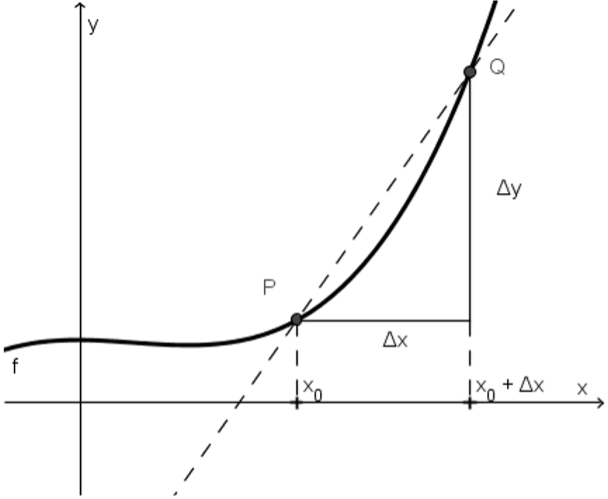
\includegraphics[width = 0.5 \textwidth]{im/differenzenquo.png}
    % \end{center}
    % 
    % Häufig wird statt $\Delta x$ auch der Buchstabe $h$ (für horizontaler Abstand) verwendet. Der Differenzenquotient lautet dann:
    % \[
    %     \frac{f(x_0+h)-f(x_0 )}{h}
    % \]
    Der Differenzenquotient entspricht der durchschnittlichen Änderungsrate der Funktion $f$ im Intervall $[x_0, x_0+h]$.
\end{deff}

Je nach Anwendung kann der Differenzenquotient die \emph{durchschnittliche} Geschwindigkeit einer Sprinterin, die \emph{durchschnittliche} Beschleunigung einer Rakete oder die \emph{durchschnittliche} Abnahmerate der Wirkstoffkonzentration pro Zeiteinheit eines Medikaments darstellen.

Ist man an der \emph{momentanen} Geschwindigkeit, Beschleunigung oder Änderungsrate interessiert, bedient man sich einer Methode, die wir in den Einführungsaufgaben mehrfach angewendet haben: Wir lassen $h$ immer kleiner werden und untersuchen das Grenzverhalten des Differenzenquotienten für $h\to 0$.

\begin{deff}[Differenzialquotient]{}
    Falls der Grenzwert
    \[
        \lim\limits_{h\to 0} \frac{f(x_0+h)-f(x_0 )}{h}
    \]
    existiert, so nennt man ihn Differenzialquotient oder (erste) Ableitung der Funktion an der Stelle $x_0$.
    % \begin{center}
    %     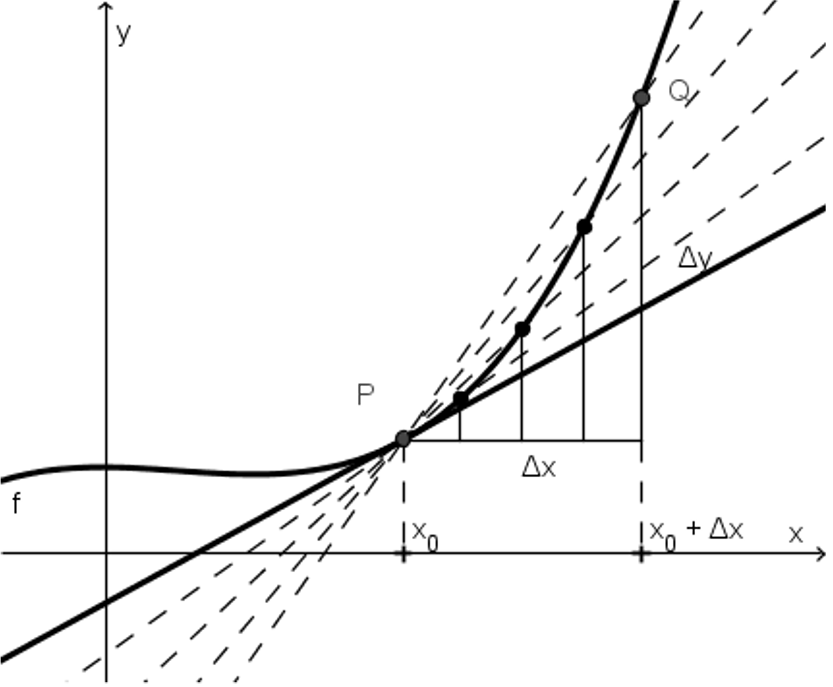
\includegraphics[width = 0.5 \textwidth]{im/differentialquo.png}
    % \end{center}

    Bezeichnungen:
    \[
        f'(x_0) \quad \text{oder} \quad \frac{d}{dx} f(x_0)
    \]
    Gesprochen: „$f$ Strich von $x_0$“ oder „$df$ nach $dx$ an der Stelle $x_0$“.

    Die Ableitung der Funktion an der Stelle $x_0$ entspricht der momentanen Änderungsrate der Funktion $f$ an der Stelle $x_0$.



\end{deff}


\begin{example}
    {Berechnung des Differenzialquotienten}{}
    Gegeben sei die Funktion $f(x)=\frac{1}{2}x^2-x$. Gesucht ist die Ableitung von $f$ an der Stelle $x_0=5$

    \kariert{26}

    % Als erstes bestimmen wir den Differenzenquotienten:
    % \begin{align*}
    %    \frac{\Delta y}{\Delta x} &= \frac{f(5+h)-f(5)}{h} \\
    %    &= \frac{\left(\frac{1}{2} (5+h)^2-(5+h) \right) - \left(\frac{1}{2}5^2 -5 \right)}{h} \\
    %    %&= \frac{\left(\frac{1}{2}(25+10h+h^2)\right)-\frac{15}{2}}{h} //
    %    &= \frac{\frac{1}{2}h^2+4h}{h}
    % \end{align*}
    % Anschliessend bilden wir den Grenzwert für $h\rightarrow0$:
    % $$f'(5) = \lim_{h\rightarrow0}\frac{\Delta y}{\Delta x}= \lim_{h\rightarrow0} \frac{\frac{1}{2}h^2+4h}{h} = \lim_{h\rightarrow0}\left(\frac{1}{2}h+4\right) = 4$$
\end{example}
%Achtung: KI generiert; bitte überprüfen und anpassen! Aufgabentypen aber ok
\subsection{Übungen}
\begin{enumerate}
    \item Berechnen Sie die durchschnittliche Änderungsrate der Funktion $f(x) = 3x^2 - 2x + 1$ im Intervall $[1, 4]$.
    \item Berechnen Sie den Differenzenquotienten der Funktion $f(x) = \sqrt{x}$ an der Stelle $x_0 = 4$ für $h = 1, 0.5, 0.1$.
    \item Berechnen Sie die Ableitung der Funktion $f(x) = 2x^2 - 5x + 3$ an der Stelle $x_0 = 2$.
    \item Berechnen Sie die Ableitung der Funktion $f(x) = \frac{1}{x}$ an der Stelle $x_0 = 1$.
\end{enumerate}
\newpage
\subsection{Geometrische Interpretation des Differenzen-/Differenzialquotienten}
% Aus Zeitgründen keine Einführungsaufgabe, sondern direkt Theorie und Übungen. Für weitere Male aber dazu eine Einführungsaufgabe mit Graphen, um die geometrische Interpretation zu verdeutlichen.
% \subsubsection{Einführungsaufgaben}
% \begin{enumerate}
%     \item Zeichnen Sie im folgenden Graphen die Sekante durch die Punkte $P(1, f(1))$ und $Q(2, f(2))$ ein. Berechnen Sie die Steigung der Sekante.
%     \item Berechnen Sie den Differenzenquotienten der Funktion im Intervall $[1,2]$. Was stellen Sie fest? Können Sie die Beobachtung begründen?
% \end{enumerate}
Der Differenzenquotient hat neben der durchschnittlichen Änderungsrate auch eine geometrische Bedeutung.

\begin{minipage}{0.6\textwidth}
    \begin{center}
        \begin{tikzpicture}[scale=1.4, >=latex]

            % Achsen
            \draw[->] (-0.5,0) -- (5.5,0) node[right] {$x$};
            \draw[->] (0,-0.5) -- (0,5.5) node[above] {$y$};

            % Funktionskurve f (kubisch-ähnlich, mit lokalem Minimum)
            \draw[thick, domain=-0.2:4.6, samples=100]
            plot (\x, {0.09*(\x-1)^3 + 0.3*(\x-1) + 1.2})
            node[left=2pt] {};

            % Funktionsname links
            \node at (0.55, 1.5) {$f$};

            % Punkte P und Q
            % P bei x0 = 2.5
            \pgfmathsetmacro{\xP}{2.5}
            \pgfmathsetmacro{\yP}{0.09*(\xP-1)^3 + 0.3*(\xP-1) + 1.2}

            % Q bei x0 + Delta_x = 4.2
            \pgfmathsetmacro{\xQ}{4.2}
            \pgfmathsetmacro{\yQ}{0.09*(\xQ-1)^3 + 0.3*(\xQ-1) + 1.2}

            % Sekante (gestrichelt), verlängert auf beiden Seiten
            \draw[dashed, thin]
            ({\xP - 1.5}, {\yP - 1.5*(\yQ-\yP)/(\xQ-\xP)})
            -- ({\xQ + 0.5}, {\yQ + 0.5*(\yQ-\yP)/(\xQ-\xP)});

            % Hilfslinie: horizontal von P bis unter Q
            \draw[thin] (\xP, \yP) -- (\xQ, \yP);

            % Hilfslinie: vertikal von Q runter auf Höhe von P
            \draw[thin] (\xQ, \yP) -- (\xQ, \yQ);

            % Delta x Beschriftung
            \node[below] at ({(\xP+\xQ)/2}, \yP) {$\Delta x$};

            % Delta y Beschriftung
            \node[right] at (\xQ, {(\yP+\yQ)/2}) {$\Delta y$};

            % Punkte P und Q einzeichnen
            \filldraw (\xP, \yP) circle (1.8pt) node[above left] {$P$};
            \filldraw (\xQ, \yQ) circle (1.8pt) node[above right] {$Q$};

            % x0 auf x-Achse
            \draw[thin] (\xP, \yP) -- (\xP, 0);
            \node[below] at (\xP, 0) {$x_0$};

            % x0 + Delta_x auf x-Achse
            \draw[thin] (\xQ, \yP) -- (\xQ, 0);
            \node[below] at (\xQ, 0) {$x_0 + \Delta x$};

        \end{tikzpicture}
    \end{center}
\end{minipage}
\begin{minipage}{0.4\textwidth}
    Steigung der Gerade durch die Punkte $P$ und $Q$ (Sekante):
    \kariert{7}
    Differenzenquotient der Funktion $f$ im Intervall $[x_0, x_0 + \Delta x]$:
    \kariert{7}
\end{minipage}
\smallskip

Ebenso hat der Differenzialquotient eine geometrische Bedeutung:

\begin{minipage}{0.6\textwidth}
    \begin{center}
        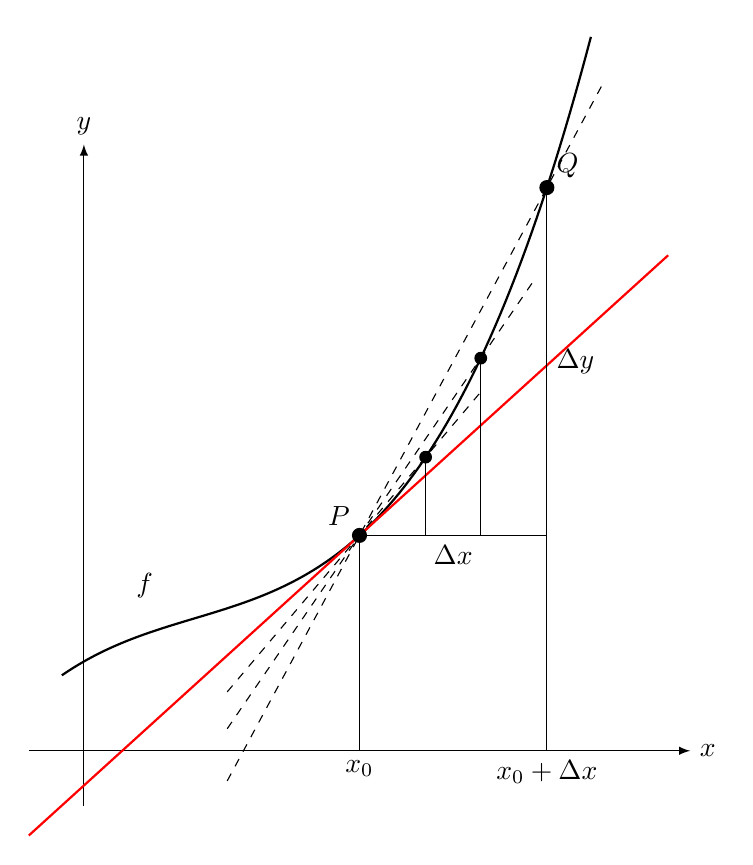
\begin{tikzpicture}[scale=1.4, >=latex]

            % Achsen
            \draw[->] (-0.5,0) -- (5.5,0) node[right] {$x$};
            \draw[->] (0,-0.5) -- (0,5.5) node[above] {$y$};

            % Funktionskurve f (kubisch-ähnlich, mit lokalem Minimum)
            \draw[thick, domain=-0.2:4.6, samples=100]
            plot (\x, {0.09*(\x-1)^3 + 0.3*(\x-1) + 1.2})
            node[left=2pt] {};

            % Funktionsname links
            \node at (0.55, 1.5) {$f$};

            % Hilfsmakro: f(x)
            % f(x) = 0.09*(x-1)^3 + 0.3*(x-1) + 1.2
            % f'(x) = 0.27*(x-1)^2 + 0.3

            % Punkt P bei x0 = 2.5
            \pgfmathsetmacro{\xP}{2.5}
            \pgfmathsetmacro{\yP}{0.09*(\xP-1)^3 + 0.3*(\xP-1) + 1.2}

            % Ableitung f'(xP) = Steigung der Tangente
            \pgfmathsetmacro{\sT}{0.27*(\xP-1)^2 + 0.3}

            % Tangente (rot), von links nach rechts
            \draw[red, thick]
            ({-0.5}, {\yP + \sT*(-0.5 - \xP)})
            -- ({5.3}, {\yP + \sT*(5.3 - \xP)});

            % Mehrere Q-Punkte und ihre Sekanten (gestrichelt)
            % xQ nimmt Werte 4.2, 3.6, 3.1 an (Q nähert sich P)
            \foreach \xQ in {4.2, 3.6, 3.1} {
                    \pgfmathsetmacro{\yQ}{0.09*(\xQ-1)^3 + 0.3*(\xQ-1) + 1.2}
                    \pgfmathsetmacro{\slope}{(\yQ-\yP)/(\xQ-\xP)}
                    % Sekante gestrichelt, über beide Seiten verlängert
                    \draw[dashed, thin]
                    ({\xP - 1.2}, {\yP - 1.2*\slope})
                    -- ({\xQ + 0.5}, {\yQ + 0.5*\slope});
                    % Senkrechter Strich vom Punkt auf der Kurve zur horizontalen Delta-x-Linie
                    \draw[thin] (\xQ, \yQ) -- (\xQ, \yP);
                    % Punkt Q_i auf der Kurve
                    \filldraw (\xQ, \yQ) circle (1.5pt);
                }

            % Outermost Q (= Q in der Vorlage) mit Label
            \pgfmathsetmacro{\xQ}{4.2}
            \pgfmathsetmacro{\yQ}{0.09*(\xQ-1)^3 + 0.3*(\xQ-1) + 1.2}

            % Hilfslinie: horizontal von P bis unter Q (nur für äusserstes Q)
            \draw[thin] (\xP, \yP) -- (\xQ, \yP);
            % Hilfslinie: vertikal von Q runter auf Höhe von P
            \draw[thin] (\xQ, \yP) -- (\xQ, \yQ);

            % Delta x / Delta y Beschriftung (nur für äusserstes Q)
            \node[below] at ({(\xP+\xQ)/2}, \yP) {$\Delta x$};
            \node[right]  at (\xQ, {(\yP+\yQ)/2}) {$\Delta y$};

            % x0 und x0+Delta_x auf x-Achse
            \draw[thin] (\xP, \yP) -- (\xP, 0);
            \node[below] at (\xP, 0) {$x_0$};
            \draw[thin] (\xQ, \yP) -- (\xQ, 0);
            \node[below] at (\xQ, 0) {$x_0 + \Delta x$};

            % Label Q für äusserstes Q
            \filldraw (\xQ, \yQ) circle (1.8pt) node[above right] {$Q$};

            % Punkt P
            \filldraw (\xP, \yP) circle (1.8pt) node[above left] {$P$};

        \end{tikzpicture}
    \end{center}
\end{minipage}
\begin{minipage}{0.4\textwidth}
    Steigung der Gerade, wenn $Q$ unendlich nahe zu $P$ kommt:
    \kariert{14}
\end{minipage}
\newpage

\begin{theo}[Geometrische Bedeutung des Differenzenquotienten]{}
    Der Differenzenquotient der Funktion $f$ im Intervall $[x_0, x_0 + \Delta x]$ entspricht der Steigung der Sekante durch die Punkte $P(x_0, f(x_0))$ und $Q(x_0 + \Delta x, f(x_0 + \Delta x))$.
\end{theo}

\begin{theo}[Geometrische Bedeutung der Ableitung an einer Stelle]{}
    Die Ableitung einer Funktion $f$ an der Stelle $x_0$ entspricht der Steigung der Tangente an den Graphen von $f$ an der Stelle $x_0$.
\end{theo}
\subsection{Übungen}
\begin{enumerate}
    \item \( f(x) = 2x^2 \)
          \begin{enumerate}
              \item  Welche Steigung hat die Sekante, welche den Graphen an den Stellen \( x = 1 \) und \( x = 2 \) schneidet?
                    %   \item Welche Steigung hat die Sekante, welche den Graphen an den Stellen \( x = 1 \) und \( x = 1 + h \) schneidet?
              \item Welche Steigung hat die Tangente, die den Graphen an der Stelle \( x = 1 \) berührt?
              \item Welche Steigung hat jene Tangente, die den Graphen an der Stelle \( x = 2 \) berührt?
          \end{enumerate}

    \item Sei \( f(x) = x^3 \).
          Berechnen Sie \( f'(2) \).

    \item Sei \( f(x) = x^2 - 5 \). Der Graph von $f$ sieht wie folgt aus:

          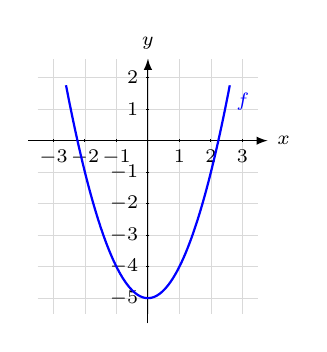
\begin{tikzpicture}[scale=0.4, >=latex,font=\scriptsize]

              % Raster (optional, kann entfernt werden)
              \draw[gray!30, very thin, step=1] (-3.5,-5.5) grid (3.5,2.6);

              % Achsen
              \draw[->] (-3.8,0) -- (3.8,0) node[right] {$x$};
              \draw[->] (0,-5.8) -- (0,2.6) node[above] {$y$};

              % Achsenbeschriftung x
              \foreach \x in {-3,-2,-1,1,2,3} {
                      \draw[thin] (\x,0.05) -- (\x,-0.05);
                      \node[below] at (\x,0) {$\x$};
                  }

              % Achsenbeschriftung y
              \foreach \y in {-5,-4,-3,-2,-1,1,2} {
                      \draw[thin] (0.05,\y) -- (-0.05,\y);
                      \node[left] at (0,\y) {$\y$};
                  }

              % Graph von f(x) = x^2 - 5
              \draw[thick, blue, domain=-2.6:2.6, samples=100]
              plot (\x, {\x*\x - 5});

              % Funktionslabel
              \node[blue, right] at (2.5, 1.25) {$f$};

          \end{tikzpicture}
          \begin{enumerate}
              \item Berechnen Sie \( f'(0) \). Welche Eigenschaft des Graphen wird durch das Resultat verdeutlicht?
              \item Berechnen Sie \( f'(2) \).
              \item Bestimmen Sie \( f'(-2) \) ohne zu rechnen, indem Sie die Symmetrie der Parabel verwenden.
          \end{enumerate}

    \item Zeichnen Sie den Graphen der Funktion \( f(x) = \frac{1}{3}x - 1 \).\\
          Entscheiden Sie ohne zu rechnen: Wie gross sind \( \frac{d}{dx} f(1) \), \( \frac{d}{dx} f(2) \) und \( \frac{d}{dx} f(-42) \)?

          % \item Die Funktion $N(t)$ beschreibt die Anzahl Bakterien einer Bakterienkultur $t$ Tage nach Beginn des Experiments. Beschreiben Sie die Bedeutung der folgenden Grössen und geben deren Einheit an.
          %       \begin{enumerate}
          %           \item $N(10)-N(5)$
          %           \item $\frac{N(10)-N(5)}{5}$
          %           \item $\lim\limits_{h\to0}\frac{N(5+h)-N(5)}{h}$
          %       \end{enumerate}

          % \item Ein Teilchen bewegt sich mit der Geschwindigkeit $v(t) = 2t^2 - 5t + 1$ [m/s] in Abhängigkeit von der Zeit $t$ [s]. Berechnen Sie die momentane Beschleunigung des Teilchens zum Zeitpunkt $t=1$.

          %       Bestimmen Sie auch die momentane Geschwindigkeit zur Zeit $t=1$ und beschreiben Sie die Bewegung des Teilchens zu diesem Zeitpunkt.

          %       % \item \textbf{Achtung Doppelbrüche!}\\
          %       %       Sei \( f(x) = \frac{1}{x + 1} \). Berechne \( f'(1) \).
          %       %       x
\end{enumerate}

\clearpage
\subsubsection*{Lösungen:}


\begin{enumerate}
    \item
          \begin{enumerate}
              \item \( 6 \)
                    %   \item \( 4 + 2h \)
              \item \( 4 \)
              \item \( 8 \)
          \end{enumerate}

    \item
          \( 12 \)


    \item
          \begin{enumerate}
              \item \( f'(0) = 0 \)

                    Der Graph hat an der Stelle \( x=0 \) eine horizontale Tangente (sprich die Tangente hat Steigung $0$). Dies ist auch anhand des Graphen ersichtlich.
              \item \( f'(2) = 4 \)
              \item  \( f'(-2) = -4 \)

                    Die Tangente an der Stelle \( x=-2 \) hat die gleiche Steigung wie die Tangente an der Stelle \( x=2 \), aber mit negativem Vorzeichen. Dies liegt daran, dass die Parabel symmetrisch zur y-Achse ist.
          \end{enumerate}

    \item
          \[
              \frac{d}{dx}f(1) = \frac{1}{3}, \quad
              \frac{d}{dx}f(2) = \frac{1}{3}, \quad
              \frac{d}{dx}f(-42) = \frac{1}{3}
          \]
          Der Graph von \( f \) ist eine Gerade mit konstanter Steigung. Daher ist die Ableitung von \( f \) an jeder Stelle gleich der Steigung der Geraden selbst, also \( \frac{1}{3} \).
          % \item
          %       \begin{enumerate}
          %           \item Bevölkerungszuwachs in Anzahl Bakterien.
          %           \item \emph{Durchschnittliche} Wachstumsrate der Population zwischen dem 5 und 10 Tag in Bakterien/Tag.
          %           \item  \emph{Momentane} Wachstumsrate der Population am fünften Tag in Bakterien/Tag.
          %       \end{enumerate}
          % \item Beschleunigung des Teilchens am Zeitpunkt \( t=1 \):
          %       \[
          %           a(1) = v'(1) = -1
          %       \]
          %       Ausserdem gilt $v(1)=-2$. Bezüglich der ausgelegten Skala, welche die Position des Teilchens beschreibt, bewegt sich das Teilchen so, dass die Werte abnehmen. Wegen der negativen Beschleunigung, bewegt sich das Teilchen immer schneller in negativer Richtung.
          %       % \item
          %       %       \( f'(1) = -\frac{1}{4} \)

\end{enumerate}